\section{Management Summary}
\subsection*{Ausgangslage}
OpenStreetMap, eine online Kartenanwendung wie Google Maps, bietet Daten, die für Fussgängernavigation genutzt werden können. Dabei müssen die bestehenden Fussgängerstreifen in die Planung einbezogen werden, um eine Überquerung der Strassen zu ermöglichen. Unglücklicherweise sind nicht alle Fussgängerstreifen in OpenStreetMap erfasst, was die Fussgängernavigation erschwert, wenn nicht sogar fehlerhaft macht.

Dieses Projekt ist der Versuch einer automatischen Erkennung von Fussgängerstreifen auf Orthofotos (umgangssprachlich Satellitenbilder). Da das maschinelle Erfassen von Daten in OpenStreetMap nicht erlaubt ist, müssen die gefundenen Koordinaten in ein Crowdsourcing-System wie MapRoulette eingespeist werden. In dem bewerten Nutzer, ob die eingefügten Daten korrekt sind oder nicht.


\subsection*{Ergebnisse}
Aus diesem Projekt entstand einen Applikation für die automatische Erkennung von Fussgängerstreifen. Diese bezieht in einem angegebenen Bereich automatisch die entsprechend Orthofotos und Strasseninformationen und extrahiert die Koordinaten der Fussgängerstreifen. Die Koordinaten werden in einer Json-Datei abgelegt und können in eine Maproulette Challenge umgewandelt werden. 
\\
\begin{figure}[H]
	\centering
	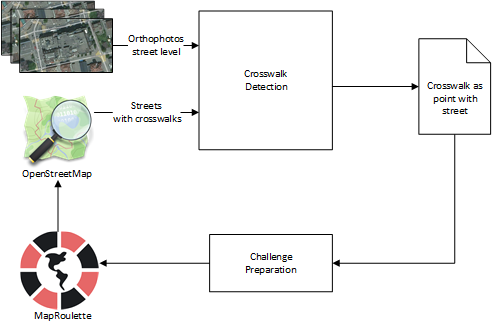
\includegraphics[]{images/management_summary_1.png}
	\caption[Management Summery Überblick]{Überblick}
\end{figure}

Diese Arbeit verwendet ein Convolutional Neuronal Network (Deep Learning) zur Klassifikation von Bildern. Die Applikation ist in einem Docker Image verfügbar. Der Erkennungprozess kann durch eine Message Queue und dem Docker Image auf verschiedene Maschinen verteilt und der Erkennungsaufwand auf mehrere Tage beschränkt werden. Ohne diese Parallelisierung hätten Wartezeiten von mehreren Wochen in Kauf genommen werden müssen.

Die Applikation erkannte mehr als 80\% aller gelben Fussgängerstreifen mit einer Fehlerrate von weniger als 10\%. Die Koordinaten der Fussgängerstreifen im Raum des Kanton Zürich, Kanton Zugs und Teile des Kanton St. Gallen konnten an Maproulette zur Einpflegung in OpenStreetMap übergeben werden.
\\
\begin{figure}[H]
	\centering
	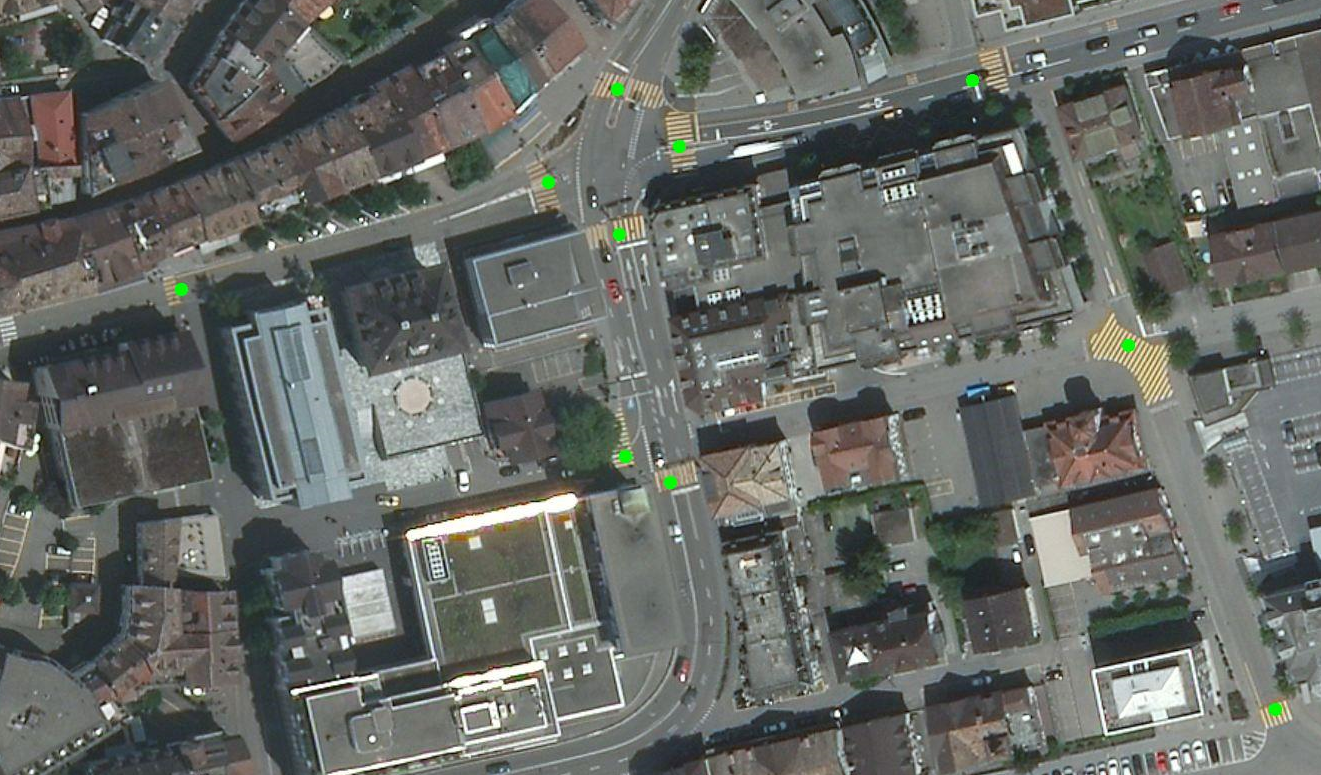
\includegraphics[width=\textwidth -10mm]{images/boxsave_rappi.png}
	\caption[Überblick]{Rapperswil Innenstadt - Gefundene Fussgängerstreifen sind mit einem grünen Punkt markiert.}
\end{figure}

\subsection*{Ausblick}
Der Erkennungsalgorithmus ist zu Ende dieses Projektes auf die Region Zürich und die Ostschweiz spezialisiert. Mit weiteren Optimierungen beim Neuronalen Netz ist es möglich, alle Fussgängerstreifen in der Schweiz zu erfassen und sogar weisse Fussgängerstreifen für andere europäische Länder zu erkennen. Auch weitere Strassenmarkierungen sind denkbar.

Weiter ist die Geschwindigkeit, in der Convolutional Neural Network verbessert werden, enorm. In 2 - 3 Jahren könnte es möglich sein, annähernd alle Fussgängerstreifen auf Orthofotos zu erkennen.
\newpage